\chapter{Онлайн алгоритм пошуку скалярного поля зсувів}\label{chapter3}

Третій розділ присвячено постановці задачi стереозору для випадку повільного надходження даних. Пропонуються алгоритми розв'язку задачі стереозору, які для такого випадку є більш ефективними, ніж алгоритми наведені в розділі \ref{chapter2}. 

Метод, описаний в підрозділі \ref{offline}, потребує наявності всіх даних до початку обчислень. В ситуації, коли дані надходять повільно, цей метод не є ефективним, адже доводиться чекати надходження всіх даних і тільки потім починати обчислення, бо ми не можемо розрахувати ваги деяких вершин.
Замість цього можна проводити деякі розрахунки з частиною даних, що вже надійшла, цим самим зменшивши час роботи алгоритму після отримання всіх даних.

\section{Постановка задачі}
Як і в частині \ref{offline}, $n$ --- довжина зображення, $I = \{1, 2, .., n\}$ --- множина координат пікселів, $D = \{0, ... , D_{max}\}$ --- множина зсувів, $D_{max}$ --- значення максимального зсуву. 
Проте ліве і праве зображення вже задаємо як функції 
\begin{align*}
	\mathcal{L} &: I \rightarrow \mathcal{C} \cup \{ \varepsilon \}, \\
	\mathcal{R} &: I \rightarrow \mathcal{C} \cup \{ \varepsilon \}.
\end{align*}

Якщо $i$-й піксель лівого зображення вже надійшов, то $ \mathcal{L}(i) $ --- інтенсивність $i$-го пікселя на лівому зображені. Якщо ще не надійшов, то $ \mathcal{L}(i) =  \varepsilon $.
Так само, як і у \ref{offline}, нам потрібно знайти таку послідовність $\overline{d} \in {D}^n$, яка мінімізує штрафну функцію \eqref{penalty}.

Цю задачу ми теж представимо як пошук найкоротшого шляху на графі $G = <\mathcal{V}, \mathcal{E}>$.
Його множина вершин, множина ребер та ваги ребер такі ж, як і в підрозділі \ref{offline_graph}. Але ваги вершин
$$v(\sigma(i, d)) = \begin{cases} h(i,d), $ якщо $  \mathcal{L}(i) \neq  \varepsilon, \\ \infty,  $ якщо $ \mathcal{L}(i) =  \varepsilon. \end{cases}$$

Будемо називати вершину $\sigma(i, d)$ \textbf{відкритою}, якщо $ \mathcal{L}(i) \neq \varepsilon$, інакше назвемо її \textbf{закритою}.

Отже, поки нам не надійшли всі дані, ми не можемо знайти таку послідовність $\overline{d} \in {D}^n$, що мінімізує штрафну функцію
$$\omega(\overline{d}) = \sum\limits_{i = 1}^n h(i, d_i) + \sum\limits_{i = 1}^{n-1} g(d_i, d_{i + 1}).$$ 
Але, щоб зменшити загальний час роботи алгоритму, ми можемо проводити деякі розрахунки з тими даними, що вже надійшли.



%%---------------------------------------------------------------------------%%
\section{Поступове упорядковане надходження даних}
Нехай на початку нам не відомі жодні пікселі обох зображень (рис. \ref{2.1nodata}),
\begin{figure}[h!]
	\centering
	\includegraphics[scale = 0.8]{allclosed2.pdf}
	\caption{Немає даних}
	\label{2.1nodata}
\end{figure}
та існує деякий стохастичний автомат, що на кожному кроці $ t \in I $ генерує пари $<c_L, \;c_R>$ --- кольори наступних пікселів лівого та правого зображень ($ c_L, c_R \in \mathcal{C} $).
Тоді на кожному кроці $ t $ нам буде відкриватися стовпчик вершин $  h(t, d), \forall d \in D, t \in I $ (рис. \ref{graphG-2}).
\begin{figure}[h!]
	\centering
	\tikzset{>=latex}
	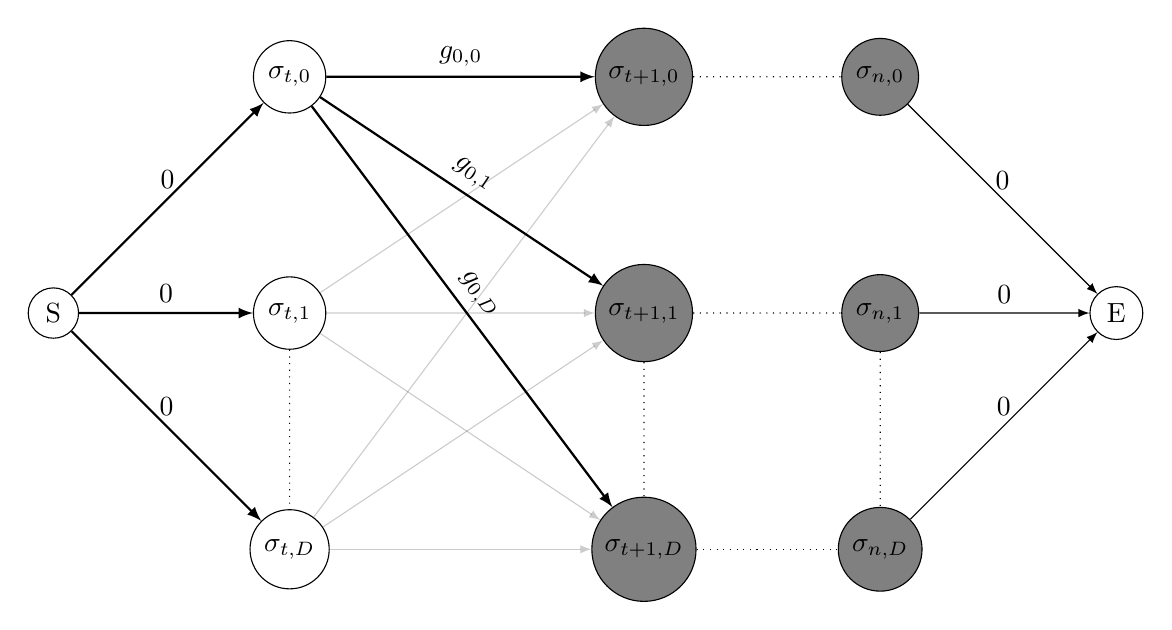
\begin{tikzpicture}[scale=1.5]
	\tikzstyle{vertex} = [circle, draw=black]
	\tikzstyle{vertex_closed_2} = [circle, draw=black, fill=gray, opacity = 30]
	\tikzstyle{vertex_opened} = [circle, draw=black]
	\tikzstyle{edge} = [->, thick]

%----------Виходить такий граф:------------------------------
	\node[vertex] (s) at (0,2) {S};
	
	\node[vertex] (v1n) at (2,0) {$\sigma_{t,D}$};
	\node[vertex] (v11) at (2,2) {$\sigma_{t,1}$};
	\node[vertex] (v10) at (2,4) {$\sigma_{t,0}$};
	
	\path[->, thick] (s) edge node[ above ] {0} (v1n);
	\path[->, thick] (s) edge node[ above ] {0} (v11);
	\path[->, thick] (s) edge node[ above ] {0} (v10);
	
	\draw[dash pattern=on \pgflinewidth off 2pt] (v11)--(v1n);
	
%------------------------------------------------------------
	\node[vertex_closed_2] (v2n) at (5,0) {$\sigma_{t+1,D}$};
	\node[vertex_closed_2] (v21) at (5,2) {$\sigma_{t+1,1}$};
	\node[vertex_closed_2] (v20) at (5,4) {$\sigma_{t+1,0}$};

	\path[->, opacity=0.2] (v11) edge node[ above,sloped ] {} (v2n);
	\path[->, opacity=0.2] (v11) edge node[ above,sloped ] {} (v21);
	\path[->, opacity=0.2] (v11) edge node[ above,sloped ] {} (v20);
	
	\path[->, opacity=0.2] (v1n) edge node[ above,sloped ] {} (v2n);
	\path[->, opacity=0.2] (v1n) edge node[ above,sloped ] {} (v21);
	\path[->, opacity=0.2] (v1n) edge node[ above,sloped ] {} (v20);
	
	%Selected
	\path[->, thick] (v10) edge node[ above,sloped ] {$g_{0,D}$} (v2n);
	\path[->, thick] (v10) edge node[ above,sloped ] {$g_{0,1}$} (v21);
	\path[->, thick] (v10) edge node[ above,sloped ] {$g_{0,0}$} (v20);
	
	\draw[dash pattern=on \pgflinewidth off 2pt] (v21)--(v2n);
	
	
%------------------------------------------------------------
	\node[vertex_closed_2] (vnn) at (7,0) {$\sigma_{n,D}$};
	\node[vertex_closed_2] (vn1) at (7,2) {$\sigma_{n,1}$};
	\node[vertex_closed_2] (vn0) at (7,4) {$\sigma_{n,0}$};


	\draw[dash pattern=on \pgflinewidth off 2pt] (v2n)--(vnn);
	\draw[dash pattern=on \pgflinewidth off 2pt] (v21)--(vn1);
	\draw[dash pattern=on \pgflinewidth off 2pt] (v20)--(vn0);
	
	\draw[dash pattern=on \pgflinewidth off 2pt] (vn1)--(vnn);
%------------------------------------------------------------
	\node[vertex] (e) at (9,2) {E};

	\path[->] (vnn) edge node[ above ] {0} (e);
	\path[->] (vn1) edge node[ above ] {0} (e);
	\path[->] (vn0) edge node[ above ] {0} (e);
	
	\end{tikzpicture}
	\caption{Граф $G$ }
	\label{graphG-2}
\end{figure}

Перед тим, як навести сам алгоритм, неформально опишемо ідею його роботи.
Припустимо, нам відомо, що найкоротший шлях з $S$ в $E$ проходить через вершину $ \sigma(t+1, d), d \in D $. 
Тоді, якщо всі вершини $ \sigma(t, d), \forall d \in D $ відкриті, ми можемо точно сказати, через яку з них буде проходити найкоротший шлях. Таку вершину назвемо \textit{оптимальною попередньою} для вершини $ \sigma(+1t, d) $. На жаль, ми не знаємо, через яку вершину $ \sigma(t+1, d), d \in D $ проходить найкоротший шлях, тож нам необхідно для кожної такої вершини знайти її оптимальну попередню вершину. Зате після цього нам вже не потрібні вершини $ \sigma(t, d), \forall d \in D $, і ми можемо їх відкинути разом з їх ребрами, замінивши на $D_{max}$ нових ребер.
Цим самим ми зменшимо загальну кількість ребер на ${D_{max}}^2$.

Нехай $G^0 = <\mathcal{V}^0, \mathcal{E}^0> = <\mathcal{V}, \mathcal{E}>$. Нехай також $ T = \{1, ..., n-1\} $ --- множина ітерацій, $ s: T \times D \rightarrow R $, $s^0(d) = 0, \; \forall d \in D $. Для відновлення послідовності 
$\overline{d}$ введемо матрицю \textit{попередніх оптимальних вершин} $\hat{\mathcal{P}}$, розмірності $n \times (D_{max} + 1)$.  $$p_{1,d} = 0, \forall d \in D. $$

Тільки-но автомат на кроці $ t \in T $ генерує нову пару $<cL, \;cR>$, шукаємо новий граф $G^t$:
\begin{enumerate}
	\item 
		$\forall d \in D :$\\
		$s^t(d) = \min\limits_{d' \in D} \big( s^{(t-1)}(d') + h(t, d') + g(d', d) \big).$\\
		$p_{t+1,d} \in \argmin\limits_{d' \in D}{\big( s^{(t-1)}(d') + h(t, d') + g(d', d) \big) }$,\\
		(якщо мінімізуючих елементів декілька, оберемо будь-який з них).
	\item 
		$\mathcal{V}^t = \mathcal{V}^{t-1} \setminus \{ \sigma(t, d) \; | \; d \in D \}.$
	\item %\begin{align*}
		Позначимо множину $ \bigcup\limits_{d \in D} <S, \sigma(t, d) > $ як $ \mathcal{A},$ \\
		множину $ \bigcup\limits_{\substack{d \in D \\ d' \in D}} <\sigma(t, d), \sigma(t+1, d') > $ як $ \mathcal{B},$ \\
		а множину $ \bigcup\limits_{d \in D} <S, \sigma(t+1, d) > $ як $ \mathcal{C}. $ Тоді 
		$$\mathcal{E}^t = \Big( \mathcal{E}^{t-1} \setminus \big( \mathcal{A} \cup \mathcal{B} \big) \Big) \cup \mathcal{C}.$$
		Вага ребра $ <S, \sigma(t+1, d) > = s^t(d)$ %, \; \forall d \in D$.
		%\end{align*}
	\item 
		$G^t = <\mathcal{V}^t, \mathcal{E}^t> $ \\
\end{enumerate}

Коли ж на кроці $ n $ автомат згенерує останні пікселі зображень, нам залишиться тільки знайти
$$ d_n = \argmin\limits_{d' \in D} \big\{ { s^{(n-D_{max}-1)}(d') + h(n, d') } \big\},$$
та відновити послідовність $\overline{d}$ через матрицю $\hat{\mathcal{P}}$
$$ d_i = p_{i+1,d_{i+1}}, i = \overline{n-1, 1}. $$

Кожен новий граф $G^t$ матиме на $(D_{max})^2$ менше ребер, ніж граф $G^{t-1}$. Таким чином, на момент приходу останніх пікселів, нам треба буде опрацювати лише $D_{max}$ ребер. Використання ж offline алгоритму потребує опрацювання $(n-1) \cdot {D_{max}}^2 $ ребер після надходження всіх даних.
А якщо б ми спочатку чекали приходу всіх даних, а тільки потім починали обчислення, нам треба було опрацювати 
$(n-1)(D_{max})^2$ ребер.

%%---------------------------------------------------------------------------%%
\section{Неупорядковане надходження даних при одному відомому зображені}
Нехай на початку нам відомі всі пікселі лише одного з зображень. Без втрати загальності припустимо, що нам відомо ліве зображення (рис. \ref{1.3nodata}).
\begin{figure}[h!]
	\centering
	\includegraphics[scale = 0.8]{allclosed.pdf}
	\caption{Немає даних}
	\label{1.3nodata}
\end{figure}
Введемо деякий стохастичний автомат, що на кожному кроці $ t \in I $ генерує пари $<i, \;c>$, де $ c $ --- інтенсивність пікселя з координатою $ i $ для невідомого зображення ($ i \in I, c \in \mathbb{R} $). 
Тоді на кожному кроці $ t $ нам буде відкриватися стовпчик вершин $  h(i, d), \forall d \in D $ (рис. \ref{graphG-2}).
\begin{figure}[h!]
	\centering
	\tikzset{>=latex}
	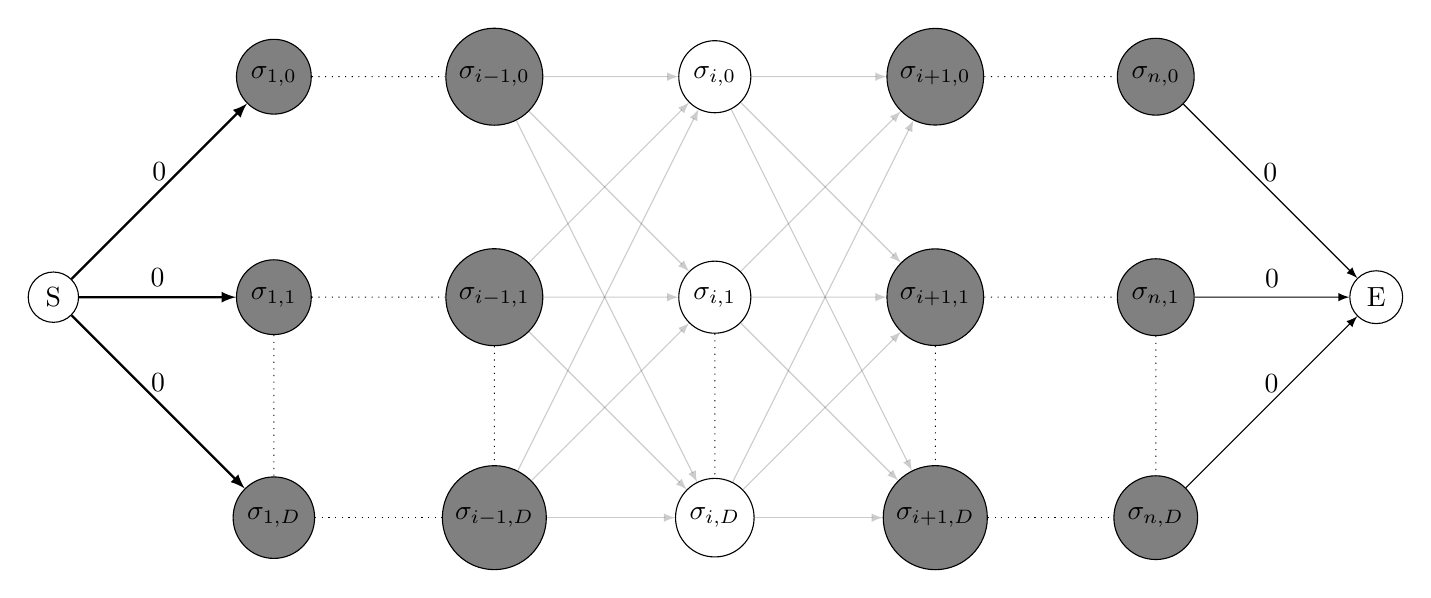
\begin{tikzpicture}[scale=1.4]
	\tikzstyle{vertex} = [circle, draw=black]
	\tikzstyle{vertex_closed_2} = [circle, draw=black, fill=gray, opacity = 30]
	\tikzstyle{vertex_opened} = [circle, draw=black]
	\tikzstyle{edge} = [->, thick]

%----------Виходить такий граф:------------------------------
	\node[vertex] (s) at (0,2) {S};
	
	\node[vertex_closed_2] (v1n) at (2,0) {$\sigma_{1,D}$};
	\node[vertex_closed_2] (v11) at (2,2) {$\sigma_{1,1}$};
	\node[vertex_closed_2] (v10) at (2,4) {$\sigma_{1,0}$};
	
	\path[->, thick] (s) edge node[ above ] {0} (v1n);
	\path[->, thick] (s) edge node[ above ] {0} (v11);
	\path[->, thick] (s) edge node[ above ] {0} (v10);
	
	\draw[dash pattern=on \pgflinewidth off 2pt] (v11)--(v1n);
	
%------------------------------------------------------------
	\node[vertex_closed_2] (v2n) at (4,0) {$\sigma_{i-1,D}$};
	\node[vertex_closed_2] (v21) at (4,2) {$\sigma_{i-1,1}$};
	\node[vertex_closed_2] (v20) at (4,4) {$\sigma_{i-1,0}$};

	\draw[dash pattern=on \pgflinewidth off 2pt] (v10)--(v20);
	\draw[dash pattern=on \pgflinewidth off 2pt] (v11)--(v21);
	\draw[dash pattern=on \pgflinewidth off 2pt] (v1n)--(v2n);
	
	\draw[dash pattern=on \pgflinewidth off 2pt] (v21)--(v2n);
	
	
%------------------------------------------------------------
	\node[vertex_opened] (v3n) at (6,0) {$\sigma_{i,D}$};
	\node[vertex_opened] (v31) at (6,2) {$\sigma_{i,1}$};
	\node[vertex_opened] (v30) at (6,4) {$\sigma_{i,0}$};

	\path[->, opacity=0.2] (v21) edge node[ above,sloped ] {} (v3n);
	\path[->, opacity=0.2] (v21) edge node[ above,sloped ] {} (v31);
	\path[->, opacity=0.2] (v21) edge node[ above,sloped ] {} (v30);
	
	\path[->, opacity=0.2] (v2n) edge node[ above,sloped ] {} (v3n);
	\path[->, opacity=0.2] (v2n) edge node[ above,sloped ] {} (v31);
	\path[->, opacity=0.2] (v2n) edge node[ above,sloped ] {} (v30);
	
	\path[->, opacity=0.2] (v20) edge node[ above,sloped ] {} (v3n);
	\path[->, opacity=0.2] (v20) edge node[ above,sloped ] {} (v31);
	\path[->, opacity=0.2] (v20) edge node[ above,sloped ] {} (v30);
	
	\draw[dash pattern=on \pgflinewidth off 2pt] (v31)--(v3n);

%------------------------------------------------------------
	\node[vertex_closed_2] (v4n) at (8,0) {$\sigma_{i+1,D}$};
	\node[vertex_closed_2] (v41) at (8,2) {$\sigma_{i+1,1}$};
	\node[vertex_closed_2] (v40) at (8,4) {$\sigma_{i+1,0}$};

	\path[->, opacity=0.2] (v31) edge node[ above,sloped ] {} (v4n);
	\path[->, opacity=0.2] (v31) edge node[ above,sloped ] {} (v41);
	\path[->, opacity=0.2] (v31) edge node[ above,sloped ] {} (v40);
	
	\path[->, opacity=0.2] (v3n) edge node[ above,sloped ] {} (v4n);
	\path[->, opacity=0.2] (v3n) edge node[ above,sloped ] {} (v41);
	\path[->, opacity=0.2] (v3n) edge node[ above,sloped ] {} (v40);
	
	\path[->, opacity=0.2] (v30) edge node[ above,sloped ] {} (v4n);
	\path[->, opacity=0.2] (v30) edge node[ above,sloped ] {} (v41);
	\path[->, opacity=0.2] (v30) edge node[ above,sloped ] {} (v40);
	
	\draw[dash pattern=on \pgflinewidth off 2pt] (v41)--(v4n);

%------------------------------------------------------------
	\node[vertex_closed_2] (vnn) at (10,0) {$\sigma_{n,D}$};
	\node[vertex_closed_2] (vn1) at (10,2) {$\sigma_{n,1}$};
	\node[vertex_closed_2] (vn0) at (10,4) {$\sigma_{n,0}$};


	\draw[dash pattern=on \pgflinewidth off 2pt] (v4n)--(vnn);
	\draw[dash pattern=on \pgflinewidth off 2pt] (v41)--(vn1);
	\draw[dash pattern=on \pgflinewidth off 2pt] (v40)--(vn0);
	
	\draw[dash pattern=on \pgflinewidth off 2pt] (vn1)--(vnn);
	
%------------------------------------------------------------
	\node[vertex] (e) at (12,2) {E};

	\path[->] (vnn) edge node[ above ] {0} (e);
	\path[->] (vn1) edge node[ above ] {0} (e);
	\path[->] (vn0) edge node[ above ] {0} (e);
	
	\end{tikzpicture}
	\caption{Граф $G$ (відкриті вершини зафарбовані білим). }
	\label{graphG-2}
\end{figure}

Перед тим, як навести сам алгоритм, неформально опишемо ідею його роботи.
Припустимо, нам відомо, що найкоротший шлях з $S$ в $E$ проходить через 
вершини $ \sigma(i+1, d')$ та $\sigma(i-1,d''), \; d', d'' \in D, i \in I $. 
Коли вершини $ \sigma(i, d), \; \forall d \in D $ стають відкритими, ми можемо точно сказати, через яку з них буде він буде проходити. Проте, $ d'$ та $ d'' $ нам не відомі, тому нам необхідно для кожної пари вершини 
$ \sigma(i-1, d')$ та $  \sigma(i+1, d'') $ знайти їх оптимальну середню вершину. 
Після цього вершини $ \sigma(i, d), \forall d \in D $ нам вже не потрібні, і ми можемо їх відкинути разом з їх ребрами, замінивши на ${D_{max}}^2$ нових ребер, зменшивши загальну кількість ребер теж на ${D_{max}}^2$. 

Введемо $G^0 = <\mathcal{V}^0, \mathcal{E}^0> = <\mathcal{V}, \mathcal{E}> = G,$
$ T = \{1, ..., n-1\} $ --- множина ітерацій. На кожній ітерації $ t $ будемо замінювати граф $ G^{t-1} $ на новий граф $ G^t $, що матиме менше ребер та вершин. Введемо функцію 
$$ w : T \times E \rightarrow \mathbb{R} ,$$
де $ w^t(v_1, v_2) $ --- вага ребра $ <v_1, v_2> $ у графі $ G^t \; (<v_1, v_2> \in E^t )$. Для знаходження cусідніх стовпчиків закритих вершин у графі $ G^t $ вводимо
$$ j = i - \sum\limits_{k = 1}^{i}{ \mathds{1}(\mathcal{L}(k) \neq \varepsilon ) }$$
Для відновлення послідовності $\overline{d}$ введемо матрицю \textit{оптимальних вершин} $\hat{\mathcal{P}}$, розмірності $I \times {(D_{max} + 1)} \times {(D_{max} + 1)}$, 
$${p^i}_{d',d''} = 0, \; \forall d',d'' \in D, \forall i \in I. $$

\newpage

Як тільки автомат на кроці $ t \in T $ генерує нову пару $<i, \;c>$, шукаємо новий граф $G^t$
\begin{enumerate}
	\item
		$ j = i - \sum\limits_{k = 1}^{i}{ \mathds{1}(\mathcal{L}(k) \neq \varepsilon ) } $,\\
		$ \hat{n} = n - \sum\limits_{k = 1}^{n}{ \mathds{1}(\mathcal{L}(k) \neq \varepsilon ) } $.\\
	\item 
		Якщо $ j = 0$,
		\begin{align}
		&w^t(s, \sigma(j+1, d)) = \min\limits_{\hat{d} \in D} \big( w^{t-1}(s, \sigma(i,\hat{d})) + h(i, \hat{d}) +  w^{t-1}(\sigma(i, \hat{d}), \sigma(j+1,d)) \big),\\
		&{p^i}_{d',d''} = \argmin\limits_{\hat{d} \in D} \big( w^{t-1}(s, \sigma(i,\hat{d})) + h(i, \hat{d}) +  w^{t-1}(\sigma(i, \hat{d}), \sigma(j+1,d)) \big). 
		\end{align}
		
	\item 
		Якщо $ j = \hat{n}$,
		\begin{align}
		& w^t(\sigma(j, d) , e ) = \min\limits_{\hat{d} \in D} \big( w^{t-1}(\sigma(j, d), \sigma(i,\hat{d})) + h(i, \hat{d}) +  w^{t-1}(\sigma(i, \hat{d}), e) \big),  \\
		& {p^i}_{d',d''} = \argmin\limits_{\hat{d} \in D} \big( w^{t-1}(\sigma(j, d), \sigma(i,\hat{d})) + h(i, \hat{d}) +  w^{t-1}(\sigma(i, \hat{d}), e) \big);
		\end{align}
		
	\item 
		Якщо $ 0 < j < \hat{n}$,
		\begin{align}
		& w^t(\sigma(j, d') , \sigma(j+1, d'') ) = \\
		&\min\limits_{\hat{d} \in D} \Big( w^{t-1}(\sigma(j, d'), \sigma(i,\hat{d})) + h(i, \hat{d}) +  w^{t-1}(\sigma(i, \hat{d}), \sigma(j+1, d'') \Big);\\
		&{p^i}_{d',d''} = \argmin\limits_{\hat{d} \in D} \Big( w^{t-1}(\sigma(j, d'), \sigma(i,\hat{d})) +  h(i, \hat{d}) +  w^{t-1}(\sigma(i, \hat{d}), \sigma(j+1, d'') \Big);
		\end{align}
		
	\item 
		$\mathcal{V}^t = \mathcal{V}^{t-1} \setminus \{ \sigma(i, d) \; | \; \forall d \in D \};$\\
	\item %\begin{align*}
		Позначимо множину $ \bigcup\limits_{d \in D} <S, \sigma(i, d) > $ як $ \mathcal{A}(i),$ \\
		множину $ \bigcup\limits_{\substack{d \in D \\ d' \in D}} <\sigma(i, d), \sigma(i+1, d') > $ як $ \mathcal{B}(i),$ \\
		а множину $ \bigcup\limits_{d \in D} <S, \sigma(t+1, d) > $ як $ \mathcal{C}. $ Тоді 
		$$\mathcal{E}^t = \Big( \mathcal{E}^{t-1} \setminus \big( \mathcal{A} \cup \mathcal{B} \big) \Big) \cup \mathcal{C}.$$
		Вага ребра $ <S, \sigma(t+1, d) > = s^t(d);$ %, \; \forall d \in D$.
		%\end{align*}
	\item 
		$G^t = <\mathcal{V}^t, \mathcal{E}^t>.$ \\
\end{enumerate}

Коли ж на кроці $ n $ автомат згенерує останні пікселі зображень, нам залишиться тільки знайти
$$ d_n = \argmin\limits_{d' \in D} \big\{ { s^{(n-D_{max}-1)}(d') + h(n, d') } \big\},$$
та відновити послідовність $\overline{d}$ через матрицю $\hat{\mathcal{P}}$
$$ d_i = p_{i+1,d_{i+1}}, i = \overline{n-1, 1}. $$

Кожен новий граф $G^t$ матиме на $(D_{max})^2$ менше ребер, ніж граф $G^{t-1}$. Таким чином, на момент приходу останніх пікселів, нам треба буде опрацювати лише $D_{max}$ ребер. А якщо б ми спочатку чекали приходу всіх даних, а тільки потім починали обчислення, нам треба було опрацювати 
$(n-1)(D_{max})^2$ ребер.





















